\documentclass[a4paper]{report}
% vim: ft=tex
\usepackage[utf8]{inputenc}
\usepackage[a4paper]{geometry}
\geometry{verbose, marginparwidth=15mm, marginparsep=3mm, tmargin=25mm}
\usepackage[english,ngerman]{babel}
\usepackage[svgnames]{xcolor}
\usepackage{graphicx}
\usepackage[hyphens]{url}
\usepackage[flushmargin,hang]{footmisc}
\usepackage{hyperref}
\usepackage{xspace} % space, but not before punctuation
\usepackage[hypcap]{caption} % link to top of tables and figures, not to bottom caption
%\usepackage[parfill]{parskip} % no idented first line of each paragraph
\usepackage{amssymb} % for \checkmark
\usepackage{textgreek} % for \textMu
\usepackage{enumitem} % for \begin{itemize}[label={...}]
\usepackage[export]{adjustbox} % left/right aligned images
\usepackage{float}
\usepackage{tikz}
\usetikzlibrary{arrows,decorations.pathmorphing,backgrounds,fit,positioning,shapes.symbols,chains,shapes.geometric,shapes.arrows,calc}
\usepackage[
backend=biber,
hyperref=true,
url=true,
isbn=false,
backref=false,
% style=custom-numeric-comp,
citereset=chapter,
maxcitenames=3,
maxbibnames=100,
block=none]{biblatex}
\bibliography{main}
\hypersetup{
	unicode=true,
	pdftitle={Roadster High Availability},
	pdfsubject={Extension of a SCADA Framework to support High Availability and Security},
	pdfauthor={Patrik Wenger, Manuel Schuler},
	pdfkeywords={ruby} {zmq} {czmq} {cztop} {high availability} {security} {encryption} {UPC UA} {SCADA} {C++},
}
\usepackage{csquotes}
\usepackage{pdfpages}
\usepackage[toc,xindy]{glossaries}
\makeglossaries
\title{Roadster High Availability}
\author{Patrik Wenger, Manuel Schuler}

\usepackage{MnSymbol}
\usepackage{listings}
\lstloadlanguages{Ruby}
\lstset{language=Ruby}
\lstset{
  prebreak=\raisebox{0ex}[0ex][0ex]{\ensuremath{\hookleftarrow}},
  postbreak=\raisebox{0ex}[0ex][0ex]{\ensuremath{\rcurvearrowse\space}},
}

% custom style for Ruby listings
\lstdefinestyle{customruby}{
  belowcaptionskip=1\baselineskip,
  breaklines=true,
  frame=single,
  frameround=tttt,
  aboveskip=1\bigskipamount,
  belowskip=1\bigskipamount,
  xleftmargin=\parindent,
  language=Ruby,
  showstringspaces=false,
  basicstyle=\footnotesize\ttfamily,
  keywordstyle=\bfseries\color{green!40!black},
  commentstyle=\itshape\color{lightgray!40!black},
  identifierstyle=\color{NavyBlue},
  stringstyle=\color{red},
  captionpos=b,
}

% inline Ruby
% This style can be used within tabular. For some reason, the customruby style
% above won't work. But it has to be used like this (not using the \rb command):
%
% 	\lstinline[style=custominlineruby]{char}
%
\lstdefinestyle{custominlineruby}{
  basicstyle=\ttfamily,
  language=Ruby,
  keywordstyle=\bfseries\color{green!40!black},
  commentstyle=\itshape\color{lightgray!40!black},
  identifierstyle=\color{NavyBlue},
  stringstyle=\color{red},
  breaklines=true,
}

\newcommand{\rb}[1]{\lstinline[
  style=custominlineruby,
  basicstyle=\ttfamily,
  prebreak={},
  postbreak={}]{#1}
}

% custom style for shell command listings
\lstdefinestyle{customsh}{
  language=sh,
  showstringspaces=false,
  basicstyle=\footnotesize\ttfamily,
  breaklines=true,
  frame=single,
  frameround=tttt,
  aboveskip=1\bigskipamount,
  belowskip=1\bigskipamount,
  captionpos=b,
}

% inline shell
\newcommand{\sh}[1]{\lstinline[
  style=customsh,
  basicstyle=\ttfamily,
  prebreak={},
  postbreak={}]{#1}}

\definecolor{diffstart}{named}{Grey}
\definecolor{diffincl}{named}{Green}
\definecolor{diffrem}{named}{OrangeRed}

% diffs
\lstdefinelanguage{diff}{
  basicstyle=\ttfamily,
  frame=single,
  frameround=tttt,
  morecomment=[f][\color{diffstart}]{@@},
  morecomment=[f][\color{diffincl}]{+},
  morecomment=[f][\color{diffrem}]{-},
}
\lstdefinestyle{customdiff}{ % custom style for diff command listings
  language=diff,
  showstringspaces=false,
  basicstyle=\scriptsize\ttfamily,
  breaklines=true,
  captionpos=b,
}

\lstdefinelanguage{worddiff}{
  basicstyle=\ttfamily,
  morecomment=[s][\color{diffincl}]{\{+}{+\}},
  morecomment=[s][\color{diffrem}]{[-}{-]}
}
\lstdefinestyle{customworddiff}{ % custom style for git diff --word-diff listings
  language=worddiff,
  showstringspaces=false,
  basicstyle=\scriptsize\ttfamily,
  breaklines=true,
  captionpos=b,
}

% C/C++ listings
\lstloadlanguages{[11]C++}
\lstset{language=C++}
\lstset{
  prebreak=\raisebox{0ex}[0ex][0ex]{\ensuremath{\hookleftarrow}},
  postbreak=\raisebox{0ex}[0ex][0ex]{\ensuremath{\rcurvearrowse\space}},
}

\lstdefinestyle{customcpp}{
  belowcaptionskip=1\baselineskip,
  breaklines=true,
  frame=single,
  frameround=tttt,
  aboveskip=1\bigskipamount,
  belowskip=1\bigskipamount,
  xleftmargin=\parindent,
  language=C++,
  showstringspaces=false,
  basicstyle=\footnotesize\ttfamily,
  keywordstyle=\bfseries\color{green!40!black},
  commentstyle=\itshape\color{lightgray!40!black},
  identifierstyle=\color{NavyBlue},
  stringstyle=\color{red},
  captionpos=b,
}

% inline C++
% This style can be used within tabular. For some reason, the customcpp style
% above won't work. But it has to be used like this (not using the \cpp command):
%
% 	\lstinline[style=custominlinecpp]{char}
%
\lstdefinestyle{custominlinecpp}{
  basicstyle=\ttfamily,
  language=C++,
  keywordstyle=\bfseries\color{green!40!black},
  commentstyle=\itshape\color{lightgray!40!black},
  identifierstyle=\color{NavyBlue},
  stringstyle=\color{red},
  breaklines=true,
}

\newcommand{\cpp}[1]{\lstinline[
  style=custominlinecpp,
  basicstyle=\ttfamily,
  prebreak={},
  postbreak={}]{#1}
}


% canonical ZMQ spelling with \zmq
\newcommand\zmq{{\O}MQ\xspace}

\begin{document}
% vim: ft=tex

% general
\newacronym{HA}{HA}{high availability}
\newacronym{OPC}{OPC}{Open Platform Communications}
\newacronym{UA}{UA}{Unified Architecture}
\newacronym{RUP}{RUP}{Rational Unified Process}
\newacronym{TIPC}{TIPC}{Transparent Inter-Process Communication}
\newacronym{TCP}{TCP}{Transmission Control Protocol}
\newacronym{PGM}{PGM}{Pragmatic General Multicast}
\newacronym{MOM}{MOM}{Message Oriented Middleware}
\newacronym{BSD}{BSD}{Berkeley Software Distribution}
\newacronym{PLC}{PLC}{Programmable Logic Controller}
\newacronym{SCADA}{SCADA}{Supervisory Control and Data Acquisition}
\newacronym{DSL}{DSL}{Domain Specific Language}
\newacronym{CHP}{CHP}{Clustered Hashmap Protocol}
\newacronym{UI}{UI}{user interface}
\newacronym{FFI}{FFI}{Foreign Function Interface}
\newacronym{ZAP}{ZAP}{ZMQ Authentication Protocol}
\newacronym{SOAP}{SOAP}{Service Oriented Application Protocol}
\newacronym{VM}{VM}{virtual machine}
\newacronym{TDD}{TDD}{test-driven development}
\newacronym{CI}{CI}{continuous integration}
\newacronym{PC}{PC}{personal computer}
\newacronym{IoT}{IoT}{Internet of Things}
\newacronym{SSD}{SSD}{Solid State Disk}
\newacronym{RAID}{RAID}{redundant array of independent disks}
\newacronym{FEDRO}{FEDRO}{Federal Roads Office}
\newacronym{IETF}{IETF}{Internet Engineering Task Force}
\newacronym{RFC}{RFC}{Request for Comments}
\newacronym{IEC}{IEC}{International Electrotechnical Commission}
\newacronym{ECC}{ECC}{elliptic curve cryptography}
\newacronym{ASCII}{ASCII}{American Standard Code for Information Interchange}
\newacronym{SSH}{SSH}{Secure Shell}
\newacronym{UUID}{UUID}{Universally unique identifier}
\newacronym{OOP}{OOP}{object-oriented programming}
\newacronym{IP}{IP}{Internet Protocol}
\newacronym{NIC}{NIC}{network interface card}
\newacronym{UPS}{UPS}{uninterruptible power supply}
\newacronym{CPU}{CPU}{central processing unit}
\newacronym{VLAN}{VLAN}{Virtual Local Area Network}

% German
\newacronym{ASTRA}{ASTRA}{Bundesamt f\"ur Strassen}
\newacronym{LTA}{LTA}{Leittechnikanlage}
\newacronym{AR}{AR}{Abschnittsrechner}
\newacronym{AS}{AS}{Anlagesystem}
\newacronym{LR}{LR}{Leitrechner}

% Roadster terminology
\newacronym{DIM}{DIM}{Domain Information Model}
\newacronym{CSP}{CSP}{Clone State Protocol}
\newacronym{RMP}{RMP}{Roadster Messaging Protocols}
\newacronym{ACP}{ACP}{Application Control Protocol}
\newacronym{CSP}{CSP}{Clone State Protocol}
\newacronym{PCP}{PCP}{Peer Control Protocol}
\newacronym{SMP}{SMP}{Supress Management Protocol}
\newacronym{PDP}{PDP}{Persistent Data Protocol}

\newglossaryentry{zmq}{
	name={\zmq},
	description={High-performance \gls{MOM} and concurrency framework,
	implemented as a standalone library},
	sort={0MQ}
}
\newglossaryentry{ruby}{
	name={Ruby},
	description={An interpreted, expressive, general-purpose \gls{OOP}
	language, created by Yukihiro Matsumoto}
}
\newglossaryentry{c}{
	name={C},
	description={A compiled, imperative, very influential low-level
		programming language, invented in the early 1970s as a Unix system
		programming language. Compared to other languages, it very simple,
		knows only a handful of primitives and keywords}
}
\newglossaryentry{actor-model}{
	name={Actor Model},
	description={A mathematical model for concurrent computation where
		there is no shared state and all communication between actors
		happens through messages}
}
\newglossaryentry{zguide}{
	name={Zguide},
	description={An extensive online
		document\footnote{\url{http://zguide.zeromq.org/page:all}} describing
		best-practice patterns for \gls{zmq}}
}
\newglossaryentry{bstar}{
	name={Binary Star Pattern},
	description={A fairly simple hot-standby and failover mechanism to
		achieve high availability between two servers, described as a reliable
		request-reply pattern in the \gls{zguide}}
}
\newglossaryentry{hot-standby}{
	name={hot standby},
	description={A method of high availability by introducing redundancy,
where the secondary system is also up and running, but just does not process
requests before the primary system fails. Failover time is typically a few
seconds}
}


\newglossaryentry{clone-pattern}{
	name={Clone Pattern},
	description={A client-server protocol to share state (a list of
		key-value pairs) across multiple clients, described as a reliable
		pub-sub pattern in the \gls{zguide}}
}

\newglossaryentry{unix-domain-socket}{
	name={Unix Domain Sockets},
	description={Named pipes for extremely performant, duplex inter-process
		communication on Unix systems}
}

\newglossaryentry{case}{
	name={case},
	description={An alarm in a Roadster application that needs to be confirmed}
}

\newglossaryentry{LOG}{
	name={LOG protocol},
	description={Used within Roadster for system logging}
}

\newglossaryentry{KISS}{
	name={KISS},
	description={The design principle ``Keep it simple, stupid'', which
		favors simplicity over complexity}
}

\newglossaryentry{wrapper-facade}{
	name={wrapper fa\c{c}ade},
	description={A structural software design pattern which provides an
		object-oriented fa\c{c}ade to a low-level functional subsystem or
		library}
}

\newglossaryentry{czmq}{
	name={CZMQ},
	description={A thin abstraction layer (\gls{wrapper-facade}) for
		\gls{zmq} with some additional functionality, written in clean and
		elegant C}
}
\newglossaryentry{cztop}{
	name={CZTop},
	description={A modern, \gls{FFI} based \gls{ruby} binding for \gls{czmq}, written by Patrik Wenger}
}

\newglossaryentry{nacl}{
	name={NaCl},
	description={Networking and Cryptography Library\footnote{\url{https://nacl.cr.yp.to}}. Modern, state-of-the-art cryptography library, created by the Daniel J. Bernstein}
}

\newglossaryentry{tweetnacl}{
	name={TweetNaCl},
	description={A compact, portable reimplementation\footnote{\url{http://tweetnacl.cr.yp.to}} of the NaCl in the
form of 100 tweets, suited to be included it into one's trusted code base (as
opposed to an external dependency). Implemented Daniel J. Bernstein et al}
}
\newglossaryentry{libsodium}{
	name={libsodium},
	description={A portable and installable variant of \gls{nacl}\footnote{\url{https://libsodium.org}}}
}
\newglossaryentry{websocket}{
	name={WebSocket},
	description={A protocol for full-duplex communication between web
browsers and web servers, standardized by the \gls{IETF} as \gls{RFC} 6455 in
2011}
}

\newglossaryentry{opc-ua}{
	name={OPC UA},
	description={\gls{OPC} gls{UA}: A set of modern standards for industrial control systems, based on cross platform webservices and other modern technology}
}

\newglossaryentry{iec-104}{
	name={IEC 60870-5-104},
	description={A \gls{IEC} transmission protocol used by SCADA applications in power system automation that enables communication via standard networks}
}

\newglossaryentry{modbus-tcp}{
	name={Modbus TCP},
	description={The TCP-based variant of Modbus, a \emph{de facto}
	standard serial communication protocol used to connect electronic devices}
}
\newglossaryentry{isa95}{
	name={ISA-95},
	description={An international standard\footnote{\url{https://en.wikipedia.org/wiki/ANSI/ISA-95}} for developing an automated interface between enterprise and control systems}
}

\newglossaryentry{ddos-attack}{
	name={distributed denial-of-service attack},
	description={is an attempt to interrupt the availability of a service
by flooding it with forged requests using a large number of source systems}
}

\newglossaryentry{Z85}{
	name={Z85 armor},
	description={a space efficient, \gls{ASCII} based, string-safe variant of the Base85 binary-to-text encoding}
}

\newglossaryentry{tc}{
	name={TokyoCabinet},
	description={a library to manage a key-value store in a single file (no server involved)}
}
\newglossaryentry{stdout}{
	name={STDOUT},
	description={the standard output channel of a Unix process (file descriptor 1)}
}
\newglossaryentry{gherkin}{
	name={Gherkin},
	description={A simple language to specify feature specifications in
	steps such as Given, When, Then\footnote{\url{https://cucumber.io/docs/reference}}}
}

\newglossaryentry{CLASS}{
	name={CLASS},
	description={C Language Style for Scalability. A standard to build
	simple, but scalable C libraries.\footnote{\url{https://rfc.zeromq.org/spec:21/CLASS}}}
}

\newglossaryentry{MRI}{
	name={MRI},
	description={Matz' Ruby interpreter. The standard Ruby interpreter,
	developed under the lead of Ruby creator Yukihiro "Matz" Matsumoto}
}

\newglossaryentry{JRuby}{
	name={JRuby},
	description={A Ruby interpreter written in Java}
}

\newglossaryentry{Rubinius}{
	name={Rubinius},
	description={A modern Ruby interpreter written in Ruby and a small C++ kernel}
}

\newglossaryentry{oom-killer}{
	name={OOM killer},
	description={Out-of-memory killer. A facility in Linux that starts
	killing appropriate processes in case the main memory becomes full.}
}

% TODO
% event-driven
% asynchronous

% TODO: streamlining:

% ROUTER & DEALER
% PUSH & PULL
% PUB & SUB
% federation & node, topology/hierarchy??
% subtree (only for DIM)
% cluster (for HA)
% COMM, CORE, STORAGE, LOG, BSTAR, ...
% subnode & supernode
% HA peer
% DIM objects
% DIM replication leads to DIM synchronization (sync across all nodes)

\thispagestyle{empty}
\selectlanguage{english}

% nice looking cover page with help from https://en.wikibooks.org/wiki/LaTeX/Title_Creation
\begin{titlepage}
\centering
\begin{raggedleft}
\includegraphics[trim=10 10 10 10, clip=true, width=0.3\textwidth]{img/hsr_logo.pdf}\end{raggedleft}
\begin{raggedright}\hfill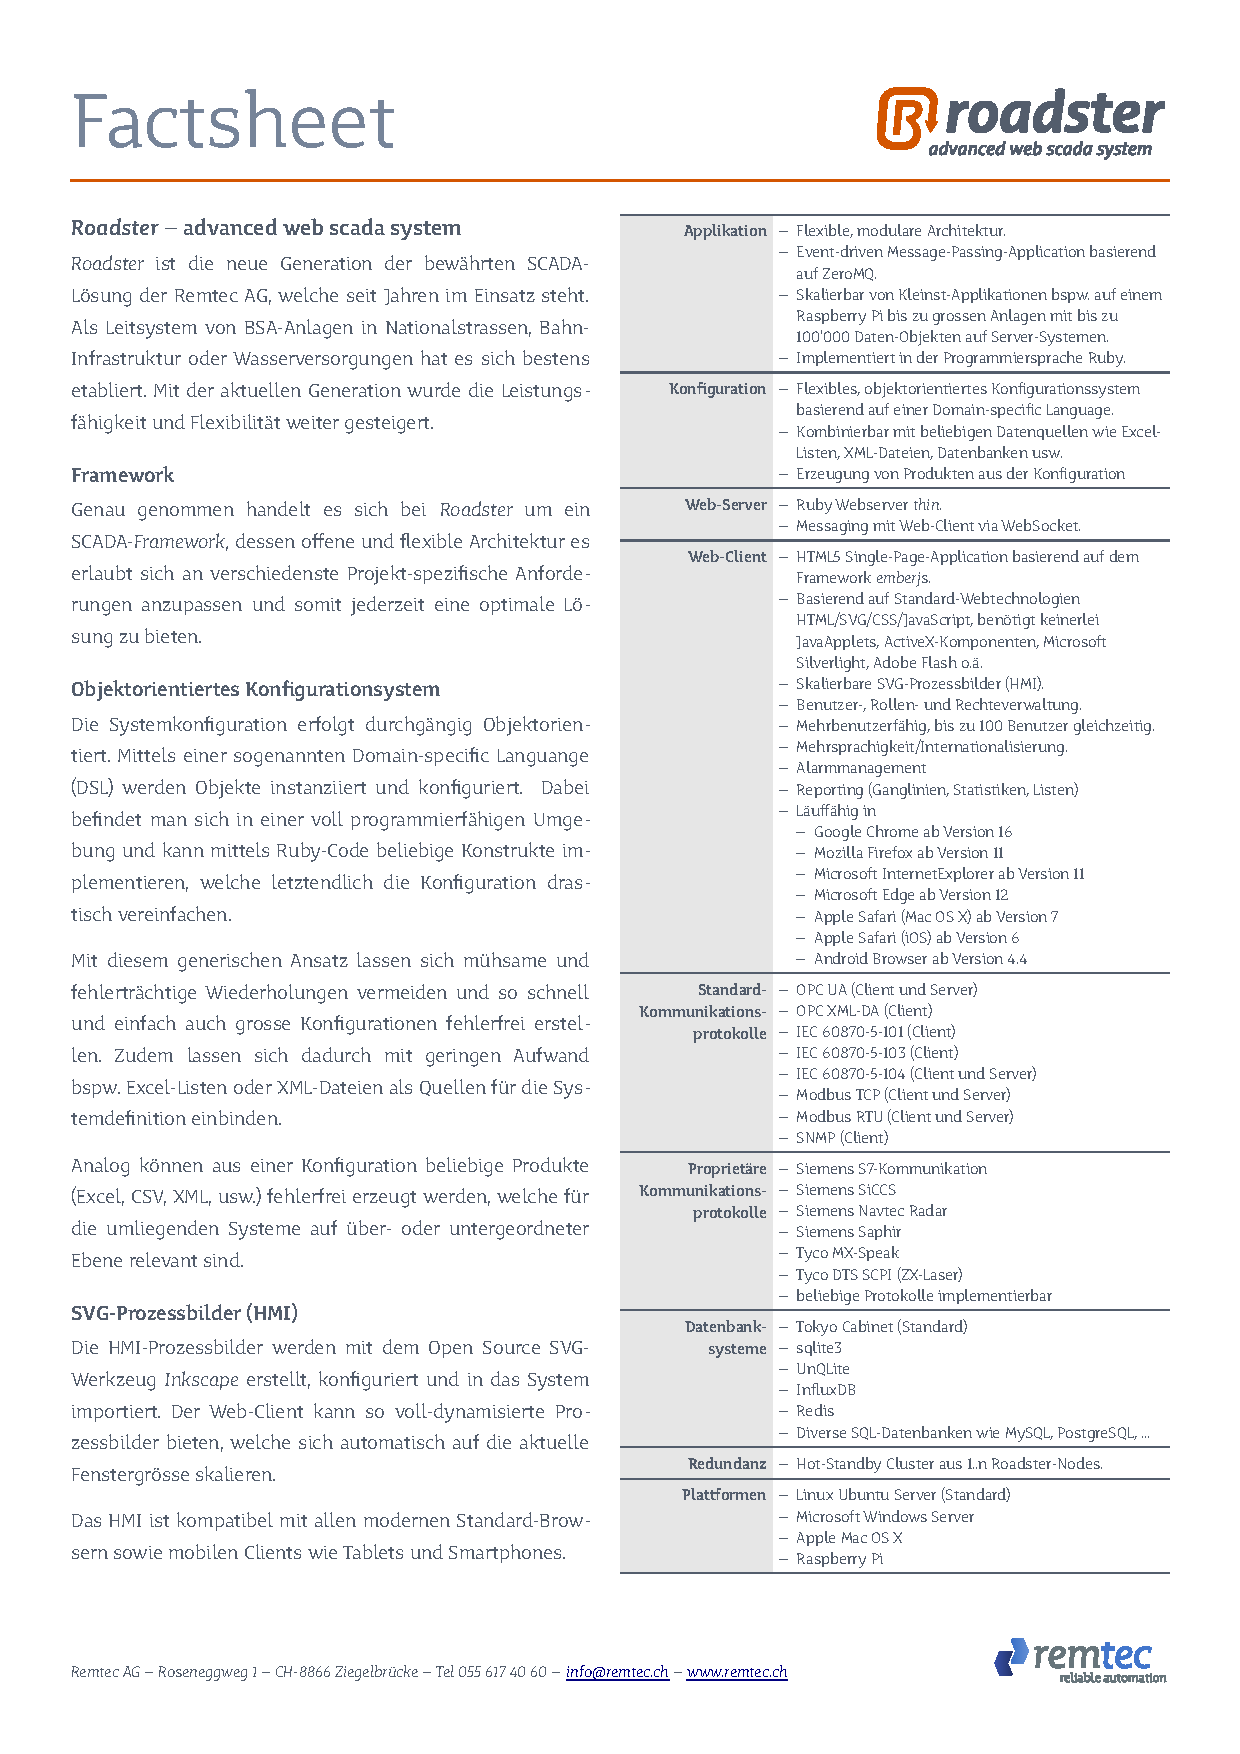
\includegraphics[trim=14.8cm 27cm 1cm 1.4cm, clip=true, width=0.38\textwidth]{img/roadster_factsheet.pdf}\end{raggedright}

\par\vspace{30mm}
{\scshape\Large Bachelor thesis\par}
\vspace{1.5cm}
{\huge\bfseries Roadster High Availability\par}
\vspace{2cm}
{\Large\itshape Patrik Wenger, Manuel Schuler\par}
\vfill
for industry client\par
mindclue GmbH
\vfill
supervised by\par
Prof. Farhad Mehta

% TODO: add name of proof reader
\vfill

% Bottom of the page
{\large Fall semester 2016\par}
\end{titlepage}

%-----------------------------------------------------------------------------
\begin{abstract}
\pagenumbering{roman}

% Introduction
TODO introduction

% Approach and Technologies
TODO approach and technologies

% Result
TODO result

\end{abstract}
%-----------------------------------------------------------------------------

\chapter*{Declaration of Originality}
We hereby confirm that we are the sole authors of this document and the
described changes to the Roadster framework and libraries developed.

TODO any usage agreements or license
%\includepdf[width=\textwidth,pages=1,pagecommand=\section{Permissions},trim=1.9cm 3cm 2cm 2cm,clip]{vereinbarung.pdf}

\chapter*{Acknoledgements}
TODO anyone we'd like to thank

%-----------------------------------------------------------------------------
% TOC, LOF, LOT, LOL
\tableofcontents
\listoffigures
\listoftables
\lstlistoflistings

\pagebreak
\pagenumbering{arabic}
\setcounter{page}{1}

%-----------------------------------------------------------------------------
\part{Management Summary}\label{part:mgmtsummary}
\part*{Management Summary}\label{part:mgmtsummary}
\setcounter{secnumdepth}{0} % avoid section numbering here

\section*{Initial Situation}
TODO describe initial situation, not too technical\\

Roadster is a next generation monitoring application.

\section*{Software Development Process}
TODO describe decision to use RUP/Scrum\\
TODO maybe describe what project management tools we'll be using\\

\section*{Personal Goals}
TODO describe personal goal: the cztop-patterns gem\\

\section*{Project Phases}
TODO describe this phase in retrospection\\

\subsection*{Inception}
TODO include Gantt chart for this phase\\
TODO describe this phase in retrospection\\

\subsection*{Elaboration}
TODO include Gantt chart for this phase\\
TODO describe this phase in retrospection\\

\subsection*{Construction}
TODO include Gantt chart for this phase\\
TODO describe this phase in retrospection\\

\subsection*{Transition}
TODO include Gantt chart for this phase\\
TODO describe this phase in retrospection\\

\section*{Results}
TODO describe results\\


%-----------------------------------------------------------------------------
\part{Technical Report}
% vim: ft=tex
\chapter{Scope}
The technical goals of this bachelor thesis include extending mindclue GmbH's
Roadster framework by adding features such as clustering, high availability and
transport security. This chapter outlines the general scope of this project.

\section{Motivation}
TODO Why do we care about this thesis? Why are we interested?\\

To better understand our motivation, it might help to understand our personal backgrounds first.

TODO: Patrik: Ruby, creation of CZTop, fascination with Actor model (e.g. Erlang, Celluloid in Ruby), interest in Pony, interest in distributed systems, huge interest in security\\
TODO: Manuel: Javascript, .NET, horizont extension, learning new things, no hesitation for this project\\

We're thrilled about the following technologies and software design patterns:

\begin{itemize}
	\item \zmq
	\item Ruby
	\item Actor Model
	\item High Availability
\end{itemize}

Coming from different backgrounds and having different degrees of experience in
each of the above technologies, we can't wait to learn more about them and put
them to actual use. The fact that the product of this bachelor thesis is most
likely going to be used in the real world only adds to the excitement.

In addition to that, we look at this bachelor thesis as an opportunity to
become more fluent in English, as well as a way to improve our skills in
crafting scientific documents using {\LaTeX}.

Depending on how we perform together as a team, further collaboration might
result in the future, either between the students themselves, or between the
students and the client. Even if not, this project will serve as a valuable
reference for future job hunting.

Last but not least, we feel like Prof. Dr. Mehta is a respected and competent
teacher whose opinions we highly value. Due to his polite parlance, discussing
project matters, both of the management and the technical kind, has always been
an enrichment.

\subsection{Open-Source Engagement}
TODO CZTop, cztop-patterns (as mentioned in the Mgmt Summary)

\section{Initial Situation}

\subsection{mindclue GmbH}
\subsubsection{About}
Die Firma mindclue GmbH mit Sitz in Ziegelbrücke GL/SG stellt für ihren
Partner REMTEC AG für Steuerungen, Regelungen und Überwachungen von technischen Prozessen,
komplette SCADA- und Steuerungssysteme her. Dabei sind sie in den Bereichen
Betriebs-und Sicherheitausrüstung für Nationalstrassen, Trinkwasser-
versorgungen, im Energiesektor und vielen Spezielbereichen tätig.
Dabei setzen sie auf ihre eigens entwickelte Applikation - Roadster.

\subsubsection{Roadster}
Roadster ist eine Ereignis gesteuerte Applikation geschrieben in Ruby.
Sie ist die eigentliche SCADA Applikation und wird bereits in einer Vielzahl von
Tunnelanlagen in der Schweiz eingesetzt und dient zur Überwachung der einzelnen Komponenten im Tunnel.
Durch den modularen Aufbau kann jede Roadster Applikation sich selbst laufen - Autonom.
Sprich jeder Roadster hat seinen eigenen Webserver und Datenverwaltung.

\subsubsection{AS - UeLS}
Roadster ist einer von vielen AS Knoten eines UeLS. Die Kommunikation
zwischen AS und AR geschieht über "OPC UA".
%TODO .... include graphics as_detail and overall system


\subsection{\zmq}
\emph{For a more detailed introduction, see \autoref{ch:zmq}.}
%TODO add acronyms/abbreviations to glossary (TIPC, TCP, PGM, MOM, BSD, NaCl, ...)
To understand Roadster's architecture and the rest of this document, it's
helpful to understand the basics of \zmq (sometimes written as ZeroMQ or simply
ZMQ) first. This is a brief introduction to \zmq for the unfamiliar reader.

\zmq is a MOM implemented as an open source library, that is, it doesn't
require a dedicated broker. Instead, it offers sockets with an abstract
interface similar to BSD sockets. Different types of sockets are used for
different messaging patterns such as request-reply, publish-subscribe, and
push-pull.

A single socket can bind/connect to multiple endpoints, which allows \zmq to
use round-robbin on the sender side, and fair-queueing on the receiver side,
where applicable. It doesn't matter whether the communication happens
in-process (between threads), inter-process (e.g. over Unix Domain Sockets), or
inter-node (e.g. over TCP/PGM/TIPC), since the transport is completely
abstracted away. The same goes for connection handling; an arbitrary amount of
connections is handled over a single socket and reconnecting after short
network failures is done transparently.

\zmq is lightweight and provides extremely low latencies, which means it can
also be used as the fabric of concurrent applications, e.g. for the actor
model. In case of the TCP transport, it incorporates advanced techniques such
as smart message batching to achieve significantly higher throughputs than with
raw TCP or other MOM solutions \cite[Figure 2, Middleware evaluation and
prototyping, p.~4]{cern:new-cmw}.

To build a solution with \zmq, its sockets are used as building blocks to
design custom message flows. Certain patterns are used to achieve reliability
with respect to the failure types that need to be addressed in particular.  The
zguide\footnote{\url{http://zguide.zeromq.org/}} explains best practices,
including commonly needed, resilient messaging patterns.

The above characteristics make \zmq a valuable asset when it comes to building
robust, distributed high-performance systems.

\subsubsection{Transport Security}
Since version 4.0, \zmq boasts state of the art encryption and authentication,
based on the excellent and highly renown
NaCl\footnote{\url{http://nacl.cr.yp.to}} library.

\subsubsection{Data Serialization}
Data serialization is outside the scope of \zmq. To fill the gap, one typically
uses another library such as MsgPack\footnote{\url{http://msgpack.org}},
Protocol
Buffers\footnote{\url{https://developers.google.com/protocol-buffers/}}, or
even a programming language's built-in object serialization
support\footnote{such as Ruby's marshalling support:
\url{http://ruby-doc.org/core/Marshal.html}}.

\subsubsection{CZMQ}
CZMQ is a high-level abstraction layer for \zmq. It makes working with the \zmq
library more expressive and allows for better portability. It also provides
additional functionality such as a reactor, a simple actor implementation, as
well as utilities for certificate and authentication handling, and LAN node
discovery. This is the recommended way of using \zmq nowadays.

\subsection{Software Architecture}
TODO more\\

Roadster is event-driven and built on the Actor model, meaning it exhibits a
shared-nothing architecture. Each Roadster node runs a number of Ruby processes
which communicate via \zmq sockets. The key here is communication:

\begin{quote}
``Don't communicate by sharing state; share state by communicating.''
\end{quote}

Running multiple, loosely coupled processes (actors) allows leveraging the full
potential of modern multi-core processors, while avoiding a whole class of
traditional concurrency problems.

Every Roadster node runs a group of actors:

\begin{description}
	\item [CORE:]
		It is responsible to start the other actors. It also plays a
		key role in keeping state in all actors synchronized, being the
		source of truth.

	\item [COMM:]
		A bunch of COMM actors communicate with the outside world of a
		node. This can be different kind of PLCs or higher level
		monitoring systems. Each COMM actor uses an adapter
		specifically written for a single communication protocol.

	\item [STORAGE:]
		This actor is used when information needs to be persisted, such
		as time series or event journals. It's the interface to a
		key-value store.

	\item [LOGGER:]
		This actor collects logging data and sends it to whatever
		target is configured, be it STDOUT, a file, or a syslog server.
\end{description}

\autoref{fig:roadster:arch} illustrates Roadster's architecture.

\begin{figure}[!ht]
	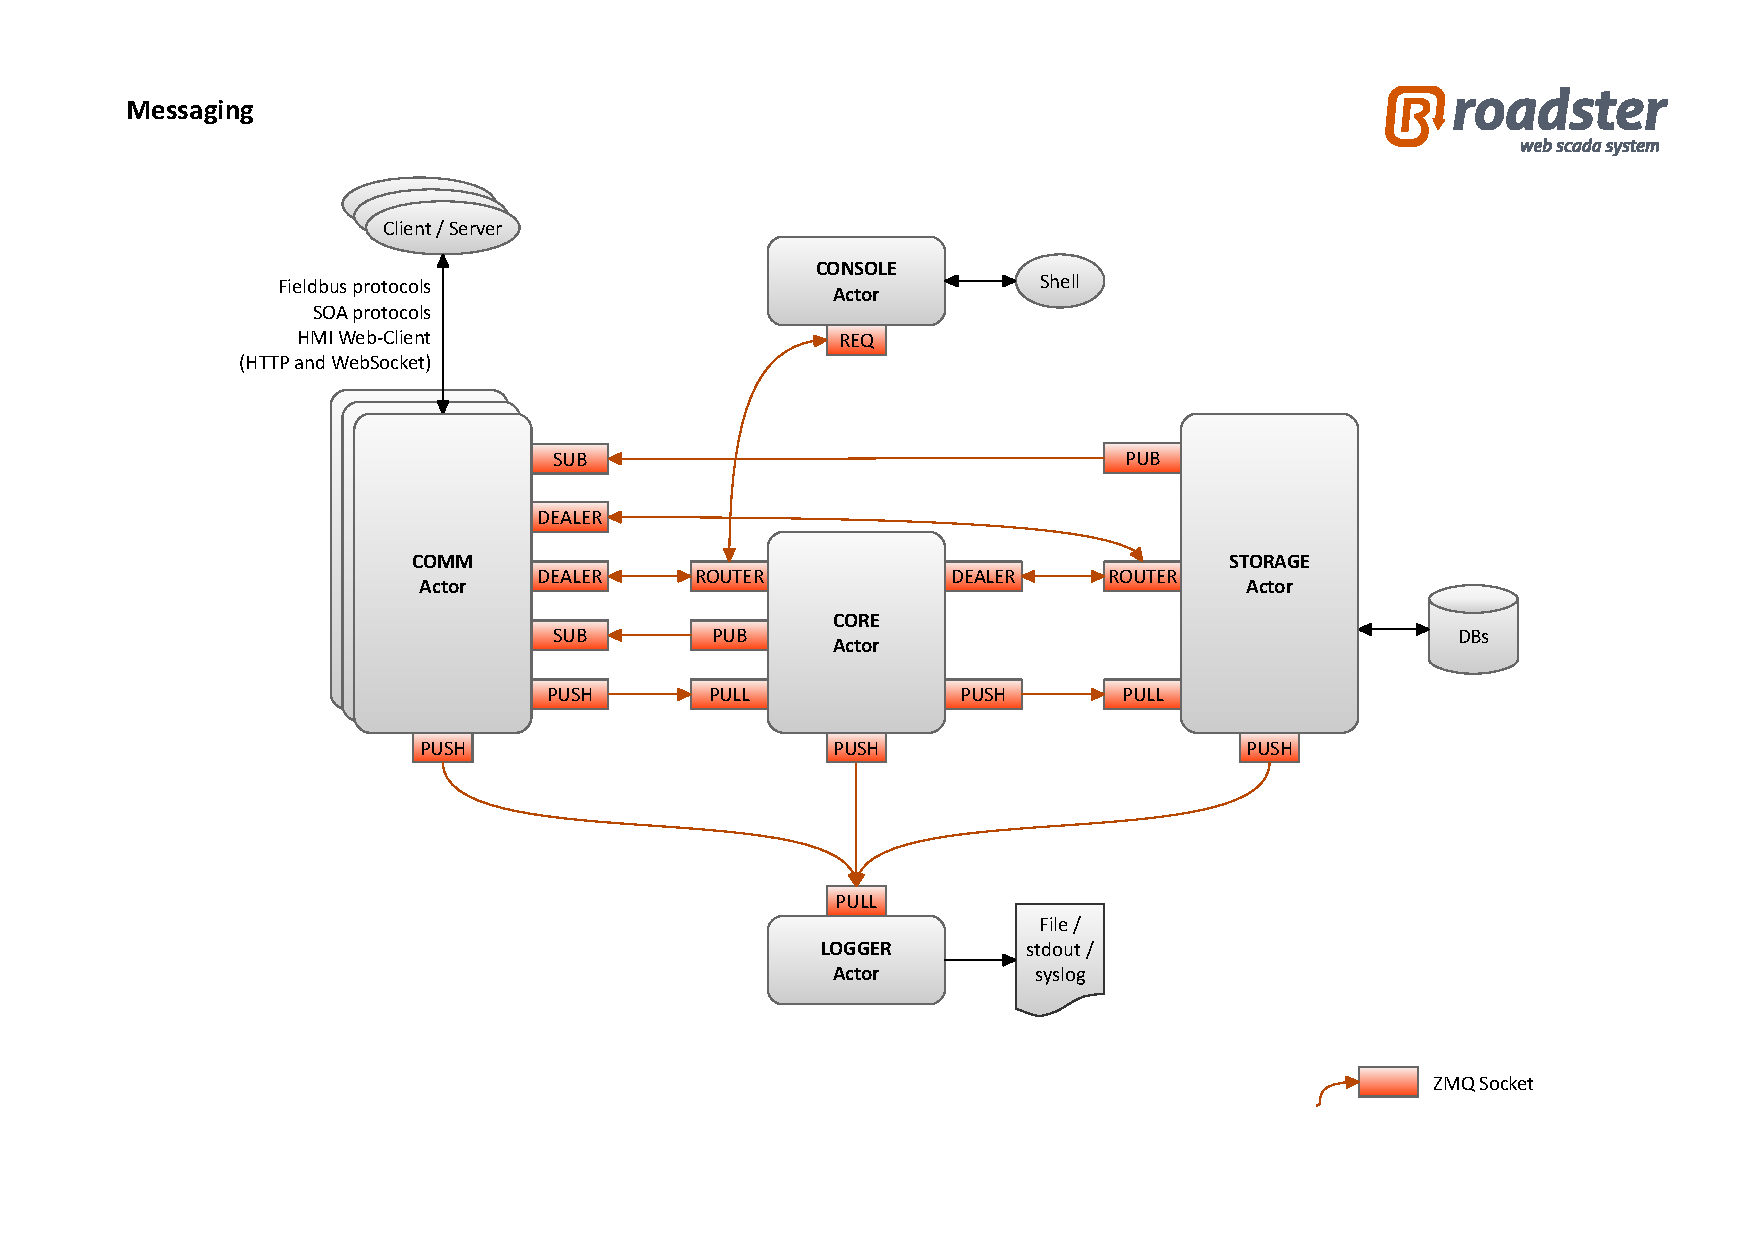
\includegraphics[trim=4cm 2cm 3.5cm 2.8cm, clip=true, width=\textwidth]{img/roadster_arch.pdf}
	\caption{Roadster's software architecture}
	\label{fig:roadster:arch}
\end{figure}

\subsubsection{Communication Layers}
TODO briefly explain layers. \autoref{fig:roadster:layers} illustrates the three layers.

\begin{figure}[!ht]
	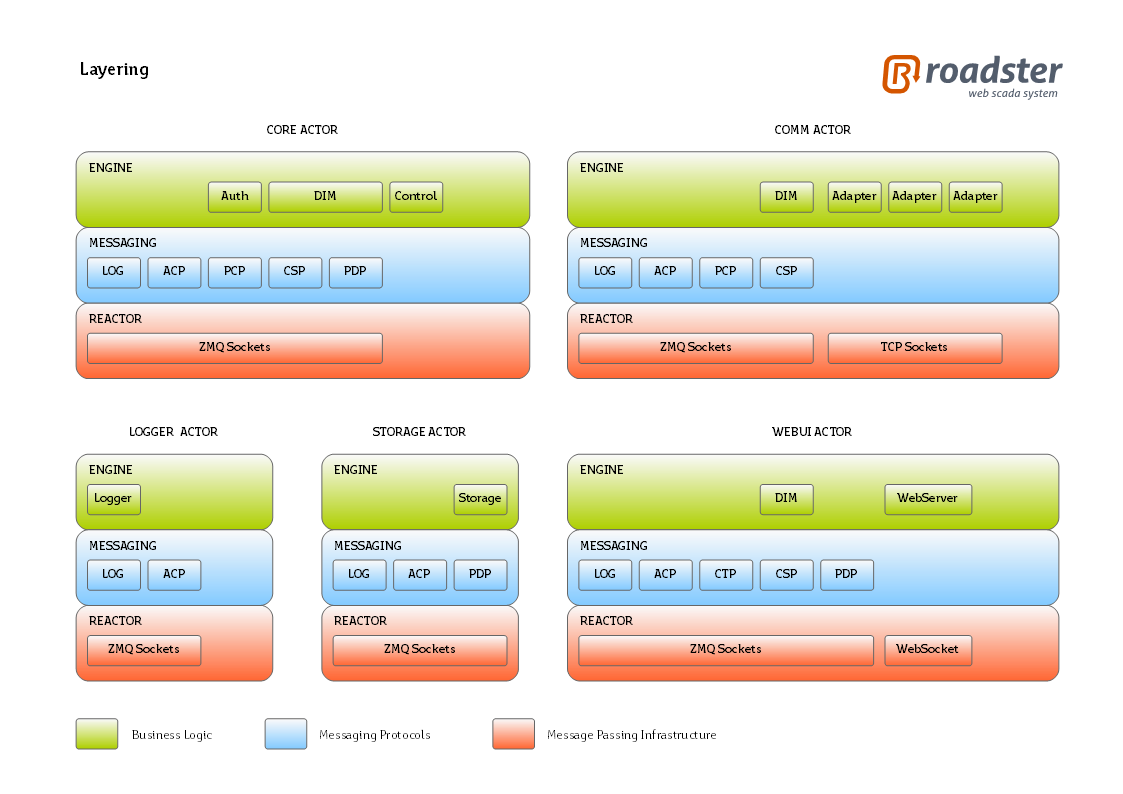
\includegraphics[trim=2cm 2.5cm 1cm 2.8cm, clip=true, width=\textwidth]{img/roadster_layering.png}
	\caption{Roadster's communication layers}
	\label{fig:roadster:layers}
TODO use PDF
\end{figure}

\section{Goals}
TODO mandatory goals

\subsection*{Optional Goals}
TODO optional goals

% vim: ft=tex
\chapter{Requirements}
TODO the requirements

\section{Priorities}
In descending priority:

\begin{enumerate}
\item multi-node CSP
\item single-level HA
\item multi-level HA
\item persistence synchronization
\item security
\item OPC UA HA (optional)
\end{enumerate}

The following sections explain the requirements in greater detail.

\section{Functional}


\subsection{Cluster}
This could also be called "Multi-node CSP".

\begin{itemize}
\item this is to allow running Roadster in a hierarchical setup
\item new COMM actors for inter node communication
\item usually 2 (or 3) levels of Roadster nodes
\item common cases:
\begin{itemize}
\item   - single level, single node (legacy)
\item   - single level HA
\item   - multi level, HA at root node only
\end{itemize}
\item exotic cases:
\begin{itemize}
\item   - multi level, HA at bottom
\item   - multi level, HA in middle
\end{itemize}
\item every subtree can live on autonomously
\item only node A has write access to values on A (to avoid uncertain situations involving race conditions), e.g.:
\begin{itemize}
\item - a forced value coming from the web UI comes through a command,
\item - routed to the relevant node, where it is applied,
\item - and then synced (up via DEALER and down via PUB, we suppose)
\end{itemize}
\item KISS
\end{itemize}


\begin{lstlisting}[style=customsh]
       C
     /   \
    A     B
\end{lstlisting}



\subsection{Single Level HA}
This is where there's a node pair directly connected to a PLC. Both nodes have read\slash write access to the PLC, but only one of the nodes (the active one) must do so. The nodes must automatically find consensus on who's active. The passive one must automatically take over in case the active one is confirmed to be dead.\\

TODO the kinds of failures we want to be able to handle: exactly hardware/software failure of the primary node, and network failure (stated by the Task Description)\\


\subsection{Multi Level HA}
This is where a node pair is the parent of one or more other nodes (subnodes).\\

TODO the kinds of failures we want to be able to handle: exactly hardware/software failure of the primary node, and network failure (stated by the Task Description)\\

\subsection{Persistence Synchronization}
This is about the synchronization of the TokyoCabinet databases. Data flow is from south to north (towards the root node), so the root node collects and maintains a replication of the persisted data of all subnodes, recursively.

\begin{itemize}
	\item autonomous
	\item not same as CHP
	\item 100\% consistency is not important
	\item data only flows from bottom to top
\end{itemize}

\subsection{Security}
\begin{itemize}
	\item transport needs to be secure (encrypted and authenticated)
	\item TODO verify requirements with Andy (we didn't really discuss this during the meeting)
	\item this requirement comes as the last mandatory goal not because it's insignificant, but because it's easy to enable transport level security on ZMQ sockets, and it would just interfere with the previous development
\end{itemize}

\subsection{OPC UA HA}
\begin{itemize}
	\item provide standardized interface upwards from HA pair
\end{itemize}

% ---------------------------------------------------------------------------
\section{Use Cases}
TODO maybe there are any?

% ---------------------------------------------------------------------------
\section{Non-Functional Requirements}
TODO the NFRs

\subsubsection{Testing}
\begin{itemize}
	\item we write unit tests for our own contributions
	\item we test the integrated result in a close-to-reality setup
\end{itemize}


\subsubsection{Coding Guidelines}
\begin{itemize}
	\item basically Ruby style guide\footnote{\url{https://github.com/bbatsov/ruby-style-guide}}
	\item method calls: only use parenthesis when needed, even with arguments (as opposed to \footnote{\url{https://github.com/bbatsov/ruby-style-guide\#method-invocation-parens}})
	\item 2 blank lines before method definition (slightly extending \footnote{\url{https://github.com/bbatsov/ruby-style-guide\#empty-lines-between-methods}})
	\item YARD API doc, 1 blank comment line before param documentation, one blank comment line before code (ignoring \footnote{\url{https://github.com/bbatsov/ruby-style-guide\#rdoc-conventions}})
	\item Ruby 1.9 symbol keys are wanted (just like \footnote{\url{https://github.com/bbatsov/ruby-style-guide\#hash-literals}})
	\item align multiple assignments so there's a column of equal signs
\end{itemize}

% vim: ft=tex
\chapter{Methodology}
TODO what have we done to arrive at the goal (should be reproducible)\\
TODO this is probably what we know as "Concept"\\



\section{Port to new ZMQ library}\label{sec:meth:port}
TODO justify why port is needed right at the beginning (exclude faults from unmaintained ffi-rzmq gem, encryption is needed anyway, all the other tasks involve communication over ZMQ)\\
TODO explain binding options out there, why CZTop (including difference between ZMQ and CZMQ)\\
TODO explain preliminary task of adding support for the ZMQ options FD and EVENTS in CZTop\\
TODO explain concept of exchanging ffi-rzmq with CZTop\\


\section{Cluster}\label{sec:meth:cluster}
TODO explain planned multi node setup\\


\begin{itemize}
	\item PCP: use DIM to know node tree and determine next hop for (dialog or fire+forget) messages
	\item decide on sync variant
	\begin{itemize}
		\item variant 1
		\begin{itemize}
			\item always sync on self-subtree only
			\item con: no copy of remaining tree
		\end{itemize}

		\item variant 2:
		\begin{itemize}
			\item always sync on complete tree
			\item get snapshot and merge own subtree
			\item (this should probably be the first step)
		\end{itemize}

		\item variant 3:
		\begin{itemize}
			\item make it configurable: either sync on subtree or complete tree
			\item (this should probably be the second step, if at all)
		\end{itemize}
	\end{itemize}
\end{itemize}


%%%%%%%%%%%%%%%%%%%%%%%%%%%%
% Actual Planning below

\subsection{DIM Synchronization}
TODO election/design of appropriate protocol\\
TODO explain Clustered Hashmap Protocol (?)\\

\begin{itemize}
	\item we need two new COMM actors
	\item they sync between super node and sub node
	\item they do something closely related to the existing CSP
	\item future oriented: because of the HA requirement, ideas from the CHP are integrated, such as using PUB-SUB (instead of PUSH-PULL) for inter-node KVSET messages, so both super nodes (in HA setup) hear updates
	\item for intra-node KVSET messages, PUSH-PULL is OK and can be left unchanged
\end{itemize}

\subsection{Node Typology Definition}

\begin{itemize}
	\item node topology in DSL, static file (e.g. topology\_conf.rb) shared on all nodes, read by each actor on startup
	\item specific config file on each node (conf.rb) knows its own place in topology (through \rb{conf.system_id})
	\item maybe a HA pair is one DIM object, has one name, but two IP addresses (primary and backup, in order)
\end{itemize}

\begin{lstlisting}[style=customruby]
# * basic method to add a node: #add_node(ID, south_facing_bind_endpoint)
# * it takes a block for defining subnodes

##################
# without HA:

conf.nodes do |map|
  map.add_node("root", "tcp://10.0.0.1:5000") do |map|
    map.add_node("subnode_a", "tcp://10.0.0.10:5000")
    map.add_node("subnode_b", "tcp://10.0.0.11:5000")
  end
end

# subnode_a can infer its endpoints from its position in the tree:
conf.system_id = "nodes.root.subnode_a"
#=> this node is "subnode_a"
#=> its IP address is 10.0.0.10
#=> north facing COMM actor's bind port is 5001
#=> south facing COMM actor's bind port is 5000
#=> north facing COMM actor will connect to "root" node on "tcp://10.0.0.1:5000"

#####################
# later with HA:

conf.nodes do |map|
  map.add_ha_pair("root", "tcp://10.0.0.1:5000", "tcp://10.0.0.2:5000") do |map|
    map.add_node("subnode_a", "tcp://10.0.0.10:5000")
    map.add_node("subnode_b", "tcp://10.0.0.11:5000")
  end
end

# subnodeA can infer its endpoints from its position in the tree:
conf.system_id = "nodes.root.subnode_a"
#=> this node is "subnode_a"
#=> its IP address is 10.0.0.10
#=> north facing COMM actor's bind port is 5001
#=> south facing COMM actor's bind port is 5000
#=> north facing COMM actor will connect to "root" HA pair on "tcp://10.0.0.1:5000" OR "tcp://10.0.0.2:5000" (Lazy Pirate algorithm)

# for primary root:
conf.system_id = "nodes.root[primary]"
\end{lstlisting}


\subsection{Message Routing}
TODO message routing (end-to-end routing with identity/identities as prepended message frame?, should be simpler and more efficient than hop-by-hop routing)\\

\section{High Availability}\label{sec:meth:ha}
TODO we have two different kinds of HA\\
TODO explain how the failures we're required to be able to handle can be handled\\
TODO expalin similarities between the two kinds of HA\\

\subsection*{Single Level}
\begin{itemize}
	\item this is different from what's described in the zguide because the concept of client requests is missing here (PLCs don't request anything)
	\item life sign from one node to the other through some continually updated PLC value
	\item mark active HA peer in DIM, OR PUSH-PULL \& different route back
	\item side note: PUSH-PULL is probably not feasible, because message are sent to inactive pull anyway, until queue full
\end{itemize}

\subsection*{Multi Level}
TODO explain why is this one different from SL-HA\\
TODO Finding consensus should be easier here, as it's closely related to the CHP described in the zguide.\\

\section{Persistence Synchronization}\label{sec:meth:psync}
\begin{itemize}
	\item super node requests for delta of TC periodically
\end{itemize}

\section{Security}\label{sec:meth:security}
TODO briefly describe ZMQ's security features, what's left for us to decide (key destribution)\\
TODO how it can be verified (-> using wireshark)\\




\section{OPC UA Interface: High Availability}\label{sec:meth:opc-ua}
TODO This is the optional goal.\\
TODO explain new opportunity for OPC UA HA server\\
TODO describe whatever needs to be described\\

\begin{itemize}
	\item study standard
	\item use Andy's gem
	\item according to Andy, this should be a simple thing
\end{itemize}

% vim: ft=tex
\chapter{Results}
TODO what are the results (without discussing them)\\
TODO these is probably the "Implementation"\\

\section{Port}\label{sec:res:port}
TODO explain results here\\


\section{Cluster}\label{sec:res:cluster}
TODO explain results here\\


\section{High Availability}\label{sec:res:ha}
TODO explain results here\\

\subsection*{Single Level HA}\label{sec:res:sl-ha}
TODO explain results here\\

\subsection*{Multi Level HA}\label{sec:res:ml-ha}
TODO explain results here\\

\section{Persistence Synchronization}\label{sec:res:psync}
TODO explain results here\\

\section{Security}\label{sec:res:security}
TODO explain results here\\

\section{OPC UA Interface: High Availability}\label{sec:res:opc-ua}
TODO explain results here\\

% vim: ft=tex
\chapter{Discussion}
TODO identify potential limitations and weaknesses of the product\\
TODO potential applications (UeLS on Roadster?)\\
TODO be concise, brief, and specific\\

\chapter{Conclusion}
TODO write conclusion, we're the best and everything is awesome
TODO they should teach the actor model in APF, because ...

\printbibliography
\printglossaries

%-----------------------------------------------------------------------------
\appendix
\part{Appendix}
\chapter{Self Reflection}
TODO how did we perform, completion of goals, accuracy of estimated efforts, efficiency, resourcefulness

\chapter{Task Description}\label{ch:task-desc}
TODO here goes the printed, signed, and scanned Task Description

\chapter{License}
As stated in the task description, all of our code contributions underlie the
ISC license, which is functionally equivalent to the MIT license and the
Simplified BSD license, but uses simpler language. In addition to that, we
hereby explicitly grant mindclue GmbH unrestricted usage of all our code
contributions.

% NOTE: meeting minutes are kept online
% NOTE: time reports are kept online

\chapter{Project Plan}
TODO import project plan from wiki\\
TODO import risks from wiki\\

\section{Organization}
TODO roles, how we organize ourselves and how we communicate with each other

\chapter{\zmq}\label{ch:zmq}
TODO explain ZMQ in greater detail

TODO strong abstraction (one socket for many connections, connection handling transparent, transport and encryption transparent, no concept of peer addresses)\\
TODO brokerless/with broker, up to you\\
TODO basic patterns\\
TODO extended patterns\\
TODO not only a "MOM", but a multi threading library (Actor pattern)\\

\chapter{Infrastructural Problems}\label{ch:problems}
TODO describe serious problems here, if any

\section{Project Management Software}
TODO Github/Trello/Harvest/Everhour/Elegantt/Ganttify/Redmine\\

\end{document}
